\documentclass[12pt,a4paper]{article}
\usepackage[utf8]{inputenc}
\usepackage[T1]{fontenc}
\usepackage{amsmath}
\usepackage{amsfonts}
\usepackage{amssymb}
\usepackage{lipsum}
\usepackage{textcomp}
\usepackage{hyperref}

\usepackage{makecell} % linebreak dans une cellule
\usepackage{multicol} % twocols localement
\usepackage{vwcol} % idem mais avec largeur variable
\usepackage{color, colortbl} % colorer les tableaux
\usepackage{enumitem} % utiliser des lettres pour énumérer
\usepackage{wrapfig} % insérer des images dans dutexte
\usepackage{dashundergaps} % transformer du texte en ________
\usepackage{MnSymbol,wasysym} % smileys
\usepackage{ifthen}
\usepackage{soul} % teste barré \st

% --- geometry ---
\usepackage{geometry}
\geometry{legalpaper, margin=2cm}
% ---

% --- xcolor ---
\usepackage{xcolor}
\definecolor{lightgray}{gray}{0.9}
% ---

% --- tcolorboxes ---
\usepackage[most]{tcolorbox}
\newtcolorbox{definition}[2][]{%
  attach boxed title to top left
               = {yshift=-8pt},
  colback      = white,
  colframe     = gray,
  fonttitle    = \bfseries,
  colbacktitle = gray,
  title        = #2,#1,
  enhanced,
}
% ---


\renewcommand{\baselinestretch}{1.15} % augmenter l'interligne

\dashundergapssetup{
	teacher-gap-format=underline,
	gap-widen
}



\author{Paul Clavier}
\title{Chapitre 5 - Droites parallèles et perpendiculaires - Activité Geogebra}

\begin{document}

% --- Section & subsection renum ---
\renewcommand\thesection{\Roman{section}}
\renewcommand\thesubsection{\arabic{subsection}}
% ---

% --- Selection manuelle de la version ---
%\TeacherModeOn
% ---

% --- Selection automatique de la version ---
\ifdefined\isprof
	\TeacherModeOn
\fi

% ---



\begin{center}
	\fbox{\parbox{\dimexpr\linewidth-2\fboxsep-2\fboxrule\relax}{\centering\huge Chapitre 7 - Cercles et polygones réguliers - Activité Geogebra}}
\end{center}

Les exercices se font à l'aide du logiciel Géogébra installé sur les ordinateurs (Tous les programmes $\backslash$ Maths $\backslash$ Géogébra).

\section*{Exercice d'introduction}
Crée un nouveau document et effectue le programme de construction suivant.
\begin{itemize}
\item place les points A, B et C non alignés
\item trace le triangle ABC
\item trace le cercle de centre A passant par B
\item trace le cercle de centre C passant par B
\item place le point D à l'intersection des deux cercles que tu as tracé
\end{itemize}
Appelle le professeur pour qu'il vérifie ta figure.

\section*{Exercice 1}
Crée un nouveau document et effectue le programme de construction suivant.
\begin{itemize}
\item place les points A et B
\item trace les triangles équilatéraux ABC et ABD (indice, tu as un compas numérique)
\end{itemize}
(Bonus) Connait tu le nom du quadrilatère ACBD? \gap*{C'est un losange}\\
Appelle le professeur pour qu'il vérifie ta figure.

\section*{Exercice 2}
Crée un nouveau document et effectue le programme de construction.
Aide: en faisant clic droit sur un objet, tu peux le cacher pour ne pas surcharger ta figure. Attention à ne pas le supprimer.
\begin{itemize}
\item place les points A et B tels que AB = 5
\item trace le triangle ABC isocèle en C tel que AC = 7
\item trace le triangle BCD rectangle en C tel que CD = 8
\end{itemize}
Appelle le professeur pour qu'il vérifie ta figure.

\newpage

\section*{Exercice Bonus}
Reproduis la figure ci dessous.

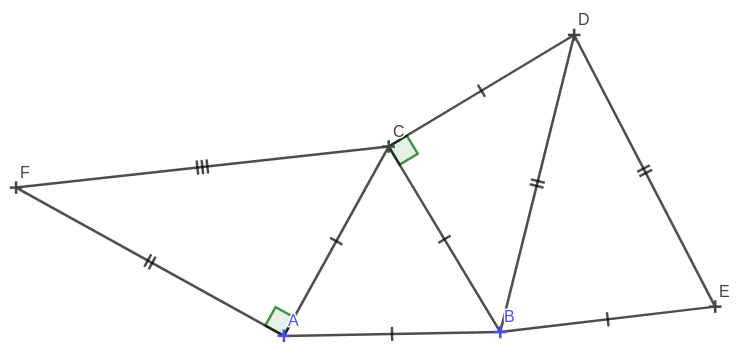
\includegraphics[scale=0.9]{img/activite-bonus.png} 

Indices: 
\begin{itemize}
\item seuls les point A et B sont libres
\item les points sont construits dans l'ordre alphabétique
\end{itemize}
\end{document}